%===============================================================================
\AufgabenHeader
%===============================================================================

%-------------------------------------------------------------------------------
\aufgabe{Elektronikgrundlagen}
%-------------------------------------------------------------------------------
\teilaufgabe
Innerhalb eines elektrischen Generators entsteht Strom, indem sich ein Magnet um
eine Drahtspule dreht. Das zugrunde liegende Prinzip nennt sich elektromagnetische
Induktion. Erklären Sie anhand folgender Abbildung, was elektrischer Stromg ist
und wie er durch das sich stets verändernde Magnetfeld erzeugt wird. Gehen Sie
dabei auch kurz das Bohrschen Atommodells ein, indem Sie die Grafik entsprechend
beschriften.

\begin{center}
    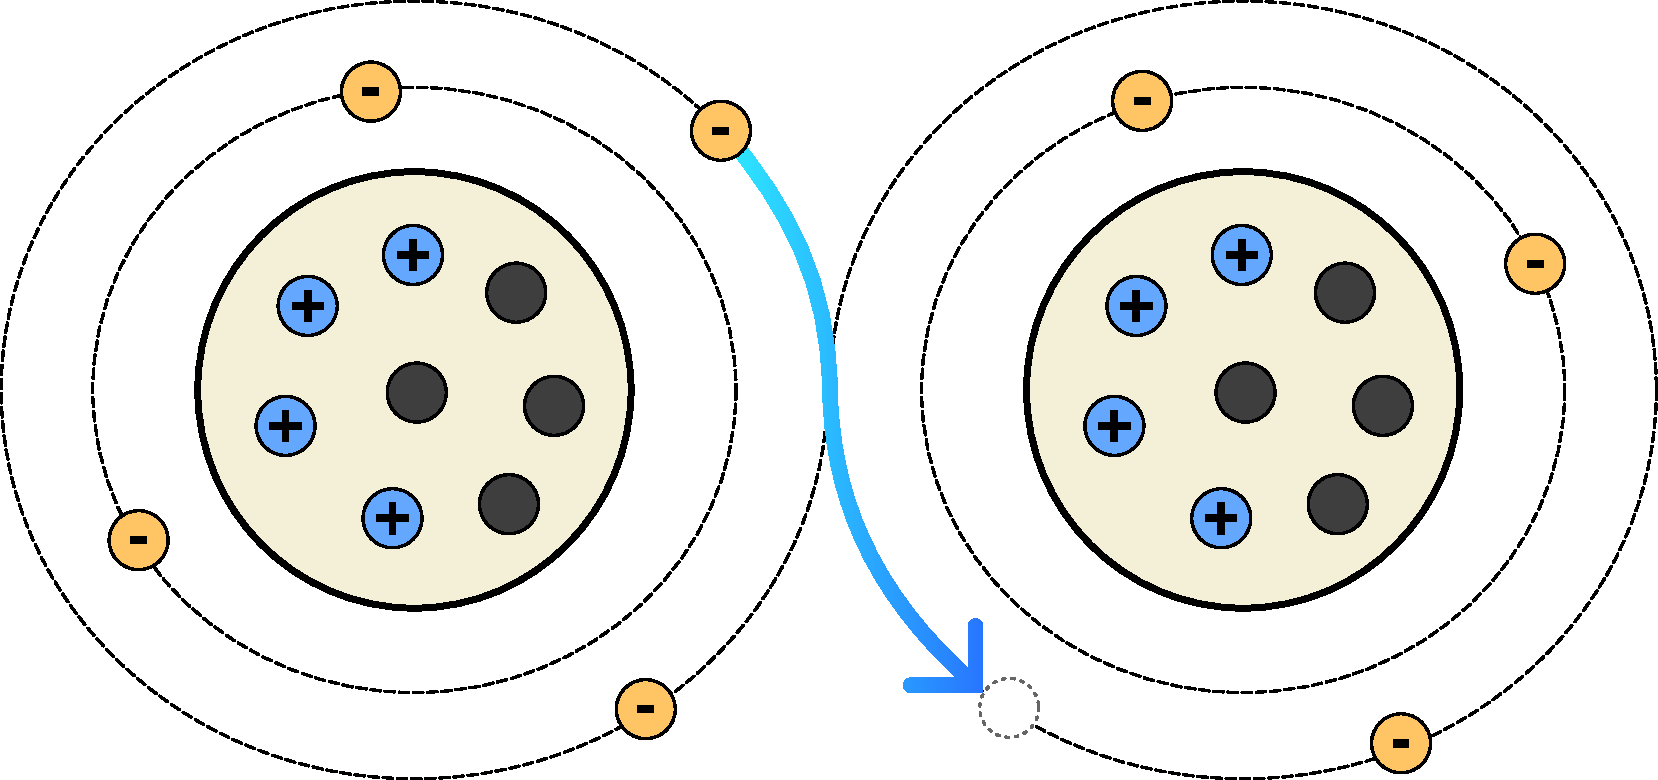
\includegraphics[width=.7\textwidth]{img/atom_elektronenfluss}
\end{center}

\bigskip
\teilaufgabe
Wann spricht man von einem Potential (auch Ladung) genannt und wann von einer
Spannung? Erklären Sie kurz, wie die beiden Begriffe zusammenhängen.

\bigskip
\teilaufgabe
Neben der Spannung sind Stromstärke, Widerstand und Leistung drei weitere
wichtige Größen der Elektrotechnik. In welchen Einheiten werden sie gemessen
und was drücken sie jeweils aus? Füllen Sie hierzu stichwortartig die folgende
Tabelle aus.

{
    \renewcommand{\arraystretch}{1.8}
    \medskip

    \begin{tabular}{|p{.15\textwidth}|p{.15\textwidth}|p{.7\textwidth}|}
        \hline
        \textbf{Kenngröße} & \textbf{Einheit} & \textbf{Bedeutung} \\
        \hline
        Spannung           &                  &                    \\[3em]
        \hline
        Stromstärke        &                  &                    \\[3em]
        \hline
        Leistung           &                  &                    \\[3em]
        \hline
        Widerstand         &                  &                    \\[3em]
        \hline
    \end{tabular}

    \medskip
}

\bigskip
\teilaufgabe
Was ist mit der Aussage gemeint, dass elektrische Schaltungen immer einen
\textbf{Stromkreis} ergeben? Und welche Bedeutung hat der Begriff \textbf{Masse}
(auf englisch Ground) damit zu tun?

\bigskip
\teilaufgabe
Die folgenden zwei Abbildungen zeigen, wie Spannung, Stromstärke, Widerstand
und Leistung in Zusammenhang stehen. Welche Größen werden durch die jeweiligen
Formelzeichen beschrieben und wie lauten die Formeln hinter den Abbildungen?

\begin{center}
    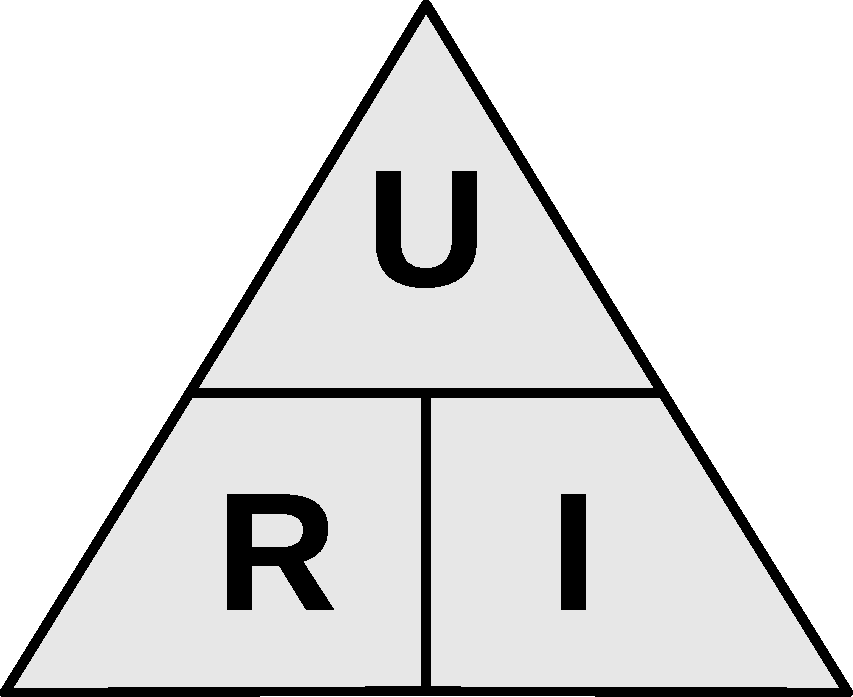
\includegraphics[width=3cm]{img/formel_uri}
    \hskip 3em
    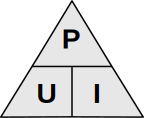
\includegraphics[width=3cm]{img/formel_pui}
\end{center}

\bigskip
\teilaufgabe
Berechnen Sie die gesuchten Werte für Widerstand, Stromstärke und Leistung in den
folgenden Anwendungsfällen:

\begin{enumerate}
    \item Für ein am Raspberry Pi anzuschließendes Bauteil beträgt die maximal
    zulässige Stromstärke 10\,mA. Welcher Vorwiderstand muss zwischen Raspberry Pi
    und Bauteil eingebaut werden?

    \item Die Spannung eines Ausgangspins am Rasbperry Pi beträgt 3,3\,V. Eine
    daran angeschlossene Leuchtdiode verringert diese entsprechend ihrer sog.
    Vorwärtsspannung um 2,2\,V. Berechnen Sie den Widerstand, der verwendet
    werden muss, um die Stromstärke auf ca. 10\,mA zu begrenzen.

    \item Ein Eingangspan des Raspberry Pi wird über einen 1k\,\si{\ohm} Widerstand
    mit einer 3,3\,V Spannungsquelle verbunden. Welche Stromstärke liegt demnach
    am Raspberry Pi an?
\end{enumerate}

\bigskip
\teilaufgabe
Wie unterscheiden sich ideale ohmsche Widerstände von Bauteilen auf Halbleiterbasis?
Warum sagt man, dass erstere einen konstanten Widerstand besitzen und letztere nicht?
Wie kann der Widerstand bei einer bestimmten Spannung anhand der Kennlinie ermittelt
werden?

%-------------------------------------------------------------------------------
\aufgabe{Strom für den Raspberry Pi}
%-------------------------------------------------------------------------------
%%% NEU
\teilaufgabe
Ein Netzteil für den Raspberry Pi wandelt Wechselstrom in Gleichstrom um und
glättet das Signal dabei. Was ist damit gemeint und warum ist das so? Erklären
Sie dabei auch, wie sich Wechselstrom und Gleichstrom unterscheiden.

\bigskip
\teilaufgabe
Ein typisches Netzteil für den Raspberry Pi funktioniert als Festspannungsnetzteil
und liefert maximal 2\,A Strom bei 5\,V Spannung. Wie viel Watt verbraucht das Netzteil
unter Volllast?

\bigskip
\teilaufgabe
Ein Schaltung auf Basis des Raspberry Pi benötigt im Schnitt 2,5\,A an Strom.
Wie lange kann diese in etwa betrieben werden, wenn ein Akkupack eine Spannung
von 5\,V mit einer Nennladung von 4\,Ah liefern kann.

\bigskip
\teilaufgabe
Ein in einem Projekt verwendeter Raspberry Pi zieht im Schnitt 3,5\,A Strom.
Welche Stromkosten entstehen nach einem Jahr Dauerbetrieb bei einem Strompreis
von 23\,Cent/kWh?

%%-------------------------------------------------------------------------------
%\aufgabe{Spannungs- und Stromteiler}
%%-------------------------------------------------------------------------------
%\teilaufgabe
%Gegeben sei eine einfache Schaltung mit drei in Reihe geschalteten Verbrauchern
%und einem Steckernetzteil als Spannungsquelle. Angenommen das Netzteil liefert
%12\,V Spannung und die Verbraucher haben die Widerstände 910\,\si{\ohm}, 750\,\si{\ohm}
%und 3k\,\si{\ohm}.

%\begin{enumerate}
    %\item Welche Teilspannungen fallen an den einzelnen Verbrauchern ab?
    %\item Wie hoch ist der Strom, der durch die Schaltung fließt?
    %\item Wie viele Kilowattstunden fallen an, wenn die Schaltung ein Jahr lang läuft?
%\end{enumerate}

%\bigskip
%\teilaufgabe
%Angenommen, die oben genannten Verbraucher wären nicht in Reihe sondern parallel
%geschaltet.

%\begin{enumerate}
    %\item Wie hoch ist der Gesamtwiderstand der Schaltung?
    %\item Welcher Gesamtstrom fließt somit durch die Schaltung?
    %\item Wie teilt sich der Gesamtstrom an den Verbrauchern auf?
%\end{enumerate}

%-------------------------------------------------------------------------------
\aufgabe{Kontakt zur Außenwelt}
%-------------------------------------------------------------------------------
\teilaufgabe
Ähnlich wie bei Software kann die Hardware eines IoT-Systems auf unterschiedlichen
Abstraktionsniveaus entworfen werden. Welche vier Arten von Hardwarebausteinen
wurden hierfür in den Folien vorgestellt? Benennen Sie diese und überlegen Sie
sich zu jeder Kategorie zwei Vor- und Nachteile.

\bigskip
\teilaufgabe
Das folgende Bild zeigt einen Raspberry Pi von oben. Beschriften Sie das Bild mit
den für gängige IoT-Anwendungen relevanten Schnittstellentechnologien.

\begin{center}
    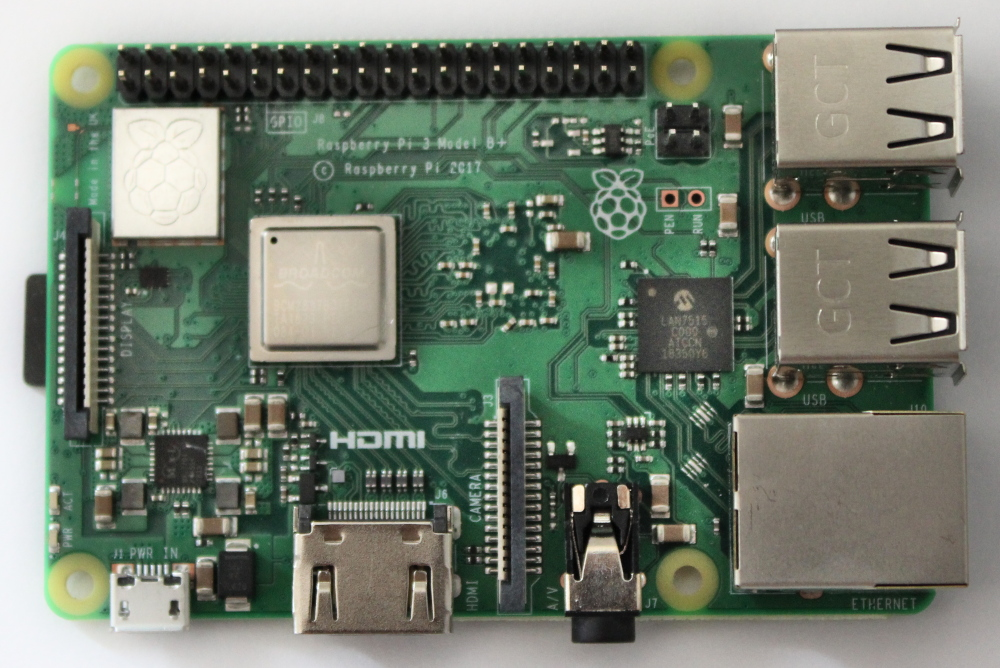
\includegraphics[width=.5\textwidth]{img/rasbperrypi_foto}
\end{center}

%%% NEU
\bigskip
\teilaufgabe
Welche Signalarten kommen grundsätzlich für die Erzeugung oder Messung durch
eingebettete Systeme in Betracht? Nennen Sie die vier in den Folien genannten
Signalarten und beschrieben Sie diese kurz.

\bigskip
\teilaufgabe
Welche Pins bietet J8-Header des Raspberry Pi? Zählen Sie alle sieben, in den
Folien genannten Arten auf.

%%%NEU
\bigskip
\teilaufgabe
Welche Grenzwerte sind bei der Verbindung von Bauteilen mit dem Raspberry Pi
unbedingt einzuhalten und wie werden sie ermittelt?

%-------------------------------------------------------------------------------
\aufgabe{Digitale Komponenten verbinden}
%-------------------------------------------------------------------------------
%\teilaufgabe
%Im letzten Aufgabenblatt haben wir integrierte Schaltkreise mit \glqq{}Chip Enable\grqq{}
%genannten Eingängen gesehen. Die anderen Ein- und Ausgänge der Bausteine müssen
%daher so genannte \glqq{}Tri-States\grqq{} sein. Recherchieren Sie den Begriff
%Tri-State und erklären Sie mit wenigen Worten, was damit gemeint ist und warum die
%kennengelernte Schaltung ohne Tri-States nicht funktionieren würde.

%%%NEU
\teilaufgabe
\textcolor{red}{
    \href{%
        https://www.falstad.com/circuit/circuitjs.html?ctz=CQAgjCAMB0l3BWcMBMcUHYMGZIA4UA2ATmIxAUgoqoQFMBaMMAKAHMRCUAWCsFTjwoo8UKCwBOnDAO7dRGQqLmiqYSizBcQi5fJB5ss-QIAmdAGYBDAK4AbAC4M7dU+DFUYkVgBlpx0S5eFTEIazsAZzoQbGhscT9CGRi8XiCU3jUQcKiYuPEpJIFsVJ0lDLE8MGJoUjr6+pZsDCpDYtLifgqITyaWgyMQEM6A916AdxARiumQyBZJ2f1phC75rQFdCraKs0tbR2dXMY9YVkWu1YF0q4T-GLRBXiNPdxzo2Pj5wuSXstE-moNJMtn8doC+q1Bn9pn8euILsVHrDSvMAEacBCEECYJDcDDEChY8QADyGigoeFoq0p8V4XQASlYIgAHNF0CQSACeAB0IgAFACWLDJlABQgQxGemCG4AEAHF+QBJADyDAAgjYImwrAA7NgimiiVZpSACVbkekCACyzKifIAFPKJAB7Gy60wASkNlHIJWxkviJUJVpAitVGq1Ov1PsglppgaGCGCcrDyrVmu1eoNGJ2mAExBKRPI8zJqVoeCQnQrylT8roAFs6BEorq6IbDITCJBsZ0u5AQ6mAMoOV0NiIOAAnEgA1nRdSwgA
    }{
        Klicken Sie hier%
    }%
}, um einen einfachen Schaltplan im CircuitJS-Onlinesimulator zu öffnen.
Untersuchen Sie die Schaltung im Simulator und beantworten Sie dann folgende Fragen
dazu:

\begin{enumerate}
    \item Werden die zulässigen Grenzwerte für den Raspberry Pi eingehalten?
    \item Warum sind die beiden LEDs in der Simulation unterschiedlich stark eingefärbt?
    \item Was passiert, wenn Sie den ersten Widerstand auf $560\,\Omega$ ändern?
    \item Wie viele weitere LEDs könnten dann mit dem Raspberry Pi verbunden werden?
\end{enumerate}

\bigskip
\teilaufgabe
Wozu werden in einer digitalen Schaltung Pull-Up- oder Pull-Down-Widerstände
genutzt. Erklären Sie kurz und ohne auf Details zur Berechnung einzugehen, wie
die Widerstände verschaltet sind und welche Aufgabe sie erfüllen.

\bigskip
\teilaufgabe
In einer Alarmanlage soll eine LED unterschiedlich schnell blinken, je nachdem
ob die Alarmanlage scharf geschaltet ist oder nicht. Im ausgeschalteten Zustand
soll die LED immer eine Sekunde lang an und eine halbe Sekunde lang aus sein.
Eingeschaltet soll sie jeweils nur eine halbe Sekunde lang an und aus sein.
Mit welchen Parametern müsste ein pulsweitenmodulierter Ausgang des Raspberry
Pi konfiguriert werden, um diese Zeitintervalle zu erreichen?

%%%NEU
\bigskip
\teilaufgabe
Wie kann ein analoger Spannungsverlauf mit dem Raspberry Pi gemessen werden,
obwohl dieser keine analogen Eingangspins besitzt?

%%%NEU
\bigskip
\teilaufgabe
Was ist eine R2R-Widerstandsleiter und wie kann sie genutzt werden, um einen
analogen Spannungsverlauf mit dem Raspberry Pi zu erzeugen?

%%%NEU
\bigskip
\teilaufgabe
Wie können stärkere Ströme, als der Raspberry Pi verträgt mit einem Transistor
oder einem Relais geschaltet werden? Zeichnen Sie jeweils einen beispielhaften
Schaltplan und erklären Sie das Prinzip daran.

%% ANS ENDE VERSCHOBEN
\bigskip
\teilaufgabe
In den Folien wurde mit einem einfachen Spannungsteiler ein 5\,V-Sensorsignal
auf für den Raspberry Pi verträgliche 3,3\,V herunter geregelt. Für solche
Aufgaben wird allerdings eher selten ein Spannungsteiler verwendet, da er ein
paar entscheidende Nachteile besitzt:

\begin{enumerate}
    \item Die Schaltung verbraucht vergleichsweise viel Strom, der als überschüssige
    Energie in Wärme umgesetzt wird.

    \item Das Schaltsignal wird durch die Schaltung zeitlich verschmiert, so dass
    nur eine begrenzte Datenrate übertragen werden kann.
\end{enumerate}

Entwerfen Sie daher eine Schaltung, die anstelle eines Spannungsteilers einen
Transistor nutzt, um den Eingangspin des Raspberry Pi mit 3,3\,V anzusteuern.
Beachten Sie dabei, dass sich bei den hier betrachteten NPN-Transistoren die
Stromstärke am Emitter (dem Ausgang des Transistors) aufsummiert. Bauen Sie
deshalb an beiden Eingängen des Transistors entsprechende Vorwiderstände ein,
um die Gesamtstromstärke auf 2\,mA zu begrenzen.

%%-------------------------------------------------------------------------------
%\aufgabe{Serielle Datenübertragung}
%%-------------------------------------------------------------------------------
%\teilaufgabe
%Die Kommunikation innerhalb eines eingebetteten Systems erfolgt oftmals über
%serielle Schnittstellen. Und wie nicht anders zu erwarten, haben unterschiedliche
%Hersteller unterschiedliche, zueinander inkompatible Standards hierfür geschaffen.
%Recherchieren Sie im Internet und füllen Sie die nachfolgende Tabelle mit den
%Eigenschaften der wichtigsten vier Standards aus:

%\newcommand{\SerialVergleich}[1]{
    %{
        %\renewcommand{\arraystretch}{1.8}
        %\newcolumntype{Y}{>{\centering\arraybackslash}X}
        %\newcolumntype{R}{>{\raggedleft\arraybackslash}p}
        %\newcolumntype{L}{>{\raggedright\arraybackslash}X}
        %\vskip \LTpre

        %\begin{tabularx}{\textwidth}{|R{.33\textwidth}|L|L|L|L|}
            %\hline
            %&
            %\textbf{UART}    &
            %\textbf{SPI}     &
            %\textbf{I²C}     &
            %\textbf{1-wire}
            %\\

            %\hline
            %\textbf{Synchron / Asynchron} &
            %\loesungswert{#1}{Asynchron} &                      % URART
            %\loesungswert{#1}{Synchron} &                       % SPI
            %\loesungswert{#1}{Synchron} &                       % I²C
            %\loesungswert{#1}{Asynchron}                        % 1-wire
            %\\[2em]

            %\hline
            %\textbf{Full-Duplex / Half-Duplex} &
            %\loesungswert{#1}{Full-Duplex} &                    % URART
            %\loesungswert{#1}{Full-Duplex} &                    % SPI
            %\loesungswert{#1}{Half-Duplex} &                    % I²C
            %\loesungswert{#1}{Half-Duplex}                      % 1-wire
            %\\[2em]

            %\hline
            %\textbf{Mehrere Empfänger möglich} &
            %\loesungswert{#1}{Nein} &                           % URART
            %\loesungswert{#1}{Ja} &                             % SPI
            %\loesungswert{#1}{Ja} &                             % I²C
            %\loesungswert{#1}{Ja}                               % 1-wire
            %\\[2em]

            %\hline
            %\textbf{Mehrere Sender möglich} &
            %\loesungswert{#1}{Nein} &                           % URART
            %\loesungswert{#1}{Ja} &                             % SPI
            %\loesungswert{#1}{Nein} &                           % I²C
            %\loesungswert{#1}{Ja}                               % 1-wire
            %\\[2em]

            %\hline
            %\textbf{Adressierung der Empfänger} &
            %\loesungswert{#1}{Keine} &                          % URART
            %\loesungswert{#1}{Slave-Select-Leitung} &           % SPI
            %\loesungswert{#1}{Adresse im Datenstrom} &          % I²C
            %\loesungswert{#1}{Adresse im Datenstrom}            % 1-wire
            %\\[2em]

            %\hline
        %\end{tabularx}

        %\vskip \LTpost
    %}
%}
%\SerialVergleich{}

%{
    %\small

    %\begin{longtable}{p{0.3\textwidth}p{0.7\textwidth}}
        %\textbf{Synchron / Asynchron:}          &  Gibt es ein Zeitsignal zur Synchronisation der Datenübertragung? \\
        %\textbf{Full-Duplex / Half-Duplex:}     &  Kann ein Bauteil gleichzeitig Daten senden und empfangen? \\
        %\textbf{Mehrere Empfänger möglich:}     &  Kann ein Sender gleichzeitig mehrere Empfänger ansprechen? \\
        %\textbf{Mehrere Sender möglich:}        &  Kann ein Bauteil von mehreren Sendern Daten empfangen? \\
        %\textbf{Adressierung der Empfänger:}    &  Wie wird ein Bauteil zum Empfang der Daten aufgefordert? \\
    %\end{longtable}
%}

%\bigskip
%\teilaufgabe
%Ein über SPI angebundener Temperatursensor sendet immer genau zwei Bytes für
%einen Temperaturwert. Das erste Byte entspricht dabei der Temperatur in Grad
%Celsius ohne Nachkommastellen, das zweite Byte liefert die Zahl hinter dem Komma.
%Zeichnen Sie ein Timingdiagramm, aus dem der zeitliche Ablauf aller Signale
%hervorgeht, wenn der Sensor den Wert 28.3 liefert.

%-------------------------------------------------------------------------------
\aufgabe{Praktische Übung}
%-------------------------------------------------------------------------------
\teilaufgabe
Die folgenden Aufgaben können direkt auf dem Raspberry Pi unter der grafischen
Desktopumgebung von Raspbian ausgeführt werden. Starten Sie daher den Rasperry
Pi und stellen Sie zunächst eine Internetverbindung her. Anschließend laden
Sie von Moodle die ZIP-Datei mit den Quellcodes dieses Kapitels herunter und
legen diese im Home-Verzeichnis des Pi ab. Danach öffnen Sie eine Kommandozeile
und führen folgenden Befehl zum Entpacken der Quellcodes aus:

\newcommand*{\CommandPrompt}[1]{\textcolor{gray}{#1}}

{
    \medskip
    \tt
    \setstretch{1.0}
    \CommandPrompt{\~{}\$} unzip Grundschaltungen.zip
    \medskip
}

Mit folgenden Befehlen können Sie dann ein neues Python Environment einrichten
und alle benötigten Zusatzbibliotheken installieren:

{
    \medskip
    \tt
    \setstretch{1.0}
    \CommandPrompt{\~{}\$} cd Grundschaltungen \\
    \CommandPrompt{\~{}/Grundschaltungen/\$} chmod +x install.sh \\
    \CommandPrompt{\~{}/Grundschaltungen/\$} ./install.sh
    \medskip
}

Zum Test können führen Sie das Beispiel \texttt{led\_blink} aus. Wenn alles gut
geht, sollten folgende Zeilen auf dem Bildschirm erscheinen:

{
    \medskip
    \tt
    \setstretch{1.0}
    \CommandPrompt{\~{}/Grundschaltungen/\$} . env/bin/activate \\
    \CommandPrompt{(env) \~{}/Grundschaltungen/\$} ./src/led\_blink.py \\
    LED ist an \\
    LED ist aus \\
    \\
    LED ist an \\
    LED ist aus \\
    \^{}C
    \medskip
}

Mit \texttt{Strg}+\texttt{C} können Sie das Programm beenden.

\bigskip
\teilaufgabe
Bauen Sie nun folgende Schaltungen aus den Folien nach und testen Sie sie mit
den entsprechenden Beispielprogrammen. Beachten Sie dabei, dass die Beispiele
immer aus der Kommandozeile heraus gestartet werden müssen und dass hierfür
wie oben gezeigt das dazugehörige Python-Environment aktiviert sein muss.

\bigskip

\begin{tabularx}{\textwidth}{|X|X|X|}
    \hline
    \textbf{Schaltung} & \textbf{Quellcodebeispiel} \\

    \hline
    LED über Widerstand direkt ansteuern &
    \verb|./src/led_blink.py| \\

    \hline
    Große Lasten über Relais schalten &
    \verb|./src/led_blink.py| \\

    \hline
    Gemittelte Leistung durch PWM regulieren &
    \verb|./src/led_pwm.py| \\
    &
    \verb|./src/led_pwm_blink.py| \\
    &
    \verb|./src/led_pwm_fade.py| \\

    \hline
    Schließkontakt mit Pull-Down-Widerstand &
    \verb|./src/button_pulldown_external.py| \\

    \hline
    Schließkontakt mit Pull-Up-Widerstand &
    \verb|./src/button_pullup_external.py| \\

    \hline
    DHT11-Sensor über 1-wire &
    \verb|./src/dht11.py| \\

    \hline
\end{tabularx}


%===============================================================================
\clearpage
\LoesungHeader
%===============================================================================

%-------------------------------------------------------------------------------
\loesung{Elektronik-Grundlagen}
%-------------------------------------------------------------------------------
\teilaufgabe
In der Abbildung gezeigte Bestandteile des bohrschen Atommodells:

\smallskip

\includegraphics[width=.5cm]{img/atom_kern}      Atomkern  \hskip 2em
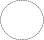
\includegraphics[width=.5cm]{img/atom_schale}    Schale    \hskip 2em

\includegraphics[width=.5cm]{img/atom_elektron}  Elektron  \hskip 2em

\includegraphics[width=.5cm]{img/atom_proton}    Proton    \hskip 2em

\includegraphics[width=.5cm]{img/atom_neutron}   Neutron

Laut dem bohrschen Atommodell besteht ein Atom aus einem Kern mit positiv geladenen
Protonen und neutralen Neutronen, um den in mehreren Bahnen (auch Schalen genannt)
negativ geladene Neutronen kreisen. Im Normalzustand besitzt das Atom dabei genauso
viele Elektronen wie Protonen. Die durch das sich drehende, magnetische Feld erzeugte
Lorentzkraft versetzt die Elektronen der äußeren Bahn (die sogenannten Valenzelektronen)
in Bewegung und sorgt so dafür, dass sie auf benachbarte Atome überspringen. Die Richtung
wird dabei durch die Bewegung des Magnetfelds vorgegeben, so dass dadurch eine gerichtete
Bewegung der Elektronen durch das leitende Material und somit ein Stromfluss entstehen.

\bigskip
\teilaufgabe
Potential oder Ladung bezeichnen den atomaren Zustand des Elektronenüberschusses
oder Elektronenmangels. Da Elektronen per Definition negativ geladen sind, besitzt
ein Atom mit zu wenigen Elektronen eine positive Ladung, da es mehr positive als
negative Ladungsträger besitzt. Umgekehrt besitzt ein Atom mit mehr Elektronen als
Protonen eine negative Ladung. Die dazugehörige Maßeinheit nennt sich Coulumb.

Die Ladung oder das Potential werden immer an einem Punkt gemessen und beziehen
sich auf den Normalzustand, indem ein Atom genauso viele Elektronen wie Protonen
besitzt und somit elektrisch neutral ist. Eine Spannung wird hingegen immer zwischen
zwei Punkten gemessen, da es sich dabei um die Ladungsdifferenz zwischen den beiden
Punkten handelt. Diese Ladungsdifferenz ist die Voraussetzung dafür, dass Strom
fließen kann, wenn die beiden Punkte über ein leitfähiges Material verbunden werden.

\bigskip
\teilaufgabe
Wichtige Bezugsgrößen der Elektrotechnik:

{
    \renewcommand{\arraystretch}{1.6}
    \medskip

    \begin{tabular}{|p{.15\textwidth}|p{.15\textwidth}|p{.7\textwidth}|}
        \hline
        \textbf{Kenngröße} &
        \textbf{Einheit}   &
        \textbf{Bedeutung} \\

        \hline
        Spannung &
        Volt &
        Beschreibt die Ladungsdifferenz zwischen zwei Punkten, vergleichbar mit
        dem Druck, den eine Pumpe auf das Wasser in einem Wasserschlauch ausübt.
        \\

        \hline
        Stromstärke &
        Ampere &
        Beschreibt wie viele Elektronen in einer gegebenen Zeit fließen, vergleichbar
        mit der Menge und Geschwindigkeit, mit der Wasser durch einen Schlauch fließt.
        \\

        \hline
        Leistung &
        Watt &
        Beschreibt die in einer Zeiteinheit verrichtete Arbeit bzw. umgesetzte Energie.
        Da der Zeitquotient bereits in der Formel für die Stromstärke enthalten ist,
        kann die Leistung einfach als Produkt aus Spannung und Strom berechnet werden.
        \\

        \hline
        Widerstand &
        Ohm &
        Ein Widerstand hindert die Bewegung der Elektronen und legt somit bei
        gegebener Spannung die erzielte Stromstärke fest. Hierfür setzt er einen
        Teil des Stroms in thermische Energie um und \glqq{}vernichtet\grqq{}
        ihn sozusagen.
        \\

        \hline
    \end{tabular}

    \medskip
}

\bigskip
\teilaufgabe
Da eine Spannung immer nur den Ladungsunterschied zwischen zwei Punkten bestimmt,
eine Spannung gleichzeitig aber auch die Ursache für den elektrischen Strom ist
(da sie die Elektronen in Bewegung setzt) benötigt jeder Stromkreis eine Quelle,
die Elektronen zur Verfügung stellt und ein Ziel, auf das sie sich zubewegen.
Die Quelle ist der Pluspol der Stromversorgung, das Ziel der Minuspol (sog.
technische Stromrichtung, tatsächlich ist es umgekehrt). Der Minuspol wird in
den meisten Fällen (wenn in der Schaltung keine negativen Spannungen benötigt
werden), gleichzeitig als Referenzpunkt für alle Spannungen definiert. Seine
Spannung beträgt per Definition daher 0\,V.

\bigskip
\teilaufgabe
Formelzeichen für die wichtigsten Berechnungen:

U = Spannung
\hskip 2em
I = Stromstärke
\hskip 2em
R = Widerstand
\hskip 2em
P = Leistung

Dazugehörige Formeln:

$U = R / I$
\hskip 2em
$R = U / I$
\hskip 2em
$I = U / R$
\hskip 6em
$P = U * I$
\hskip 2em
$U = P / I$
\hskip 2em
$I = P / U$

\bigskip
\teilaufgabe
Berechnung von Widerstand, Stromstärke und Leistung:

\begin{enumerate}
    %%
    \item Der Widerstand kann anhand der Formel $R = U / I$ berechnet werden:

    $
        R = 3,3\,V / 0,01\,A = 330\,\Omega
    $

    %%
    \item Da an der LED im Schnitt 2,2\,V der Gesamtspannung abfallen, bleiben
    nur noch 1,1\,V zur Berechnung des Widerstand übrig. Die Berechnung erfolgt
    analog zur vorherigen Teilaufgabe:

    $
        R = 1,1\,V / 0,01\,A = 110\,\Omega
    $

    %%
    \item Gemäß der Gleichung $I = U / R$ fließen $3,3\,V / 1000\,\si{\ohm} = 3,3\,mA$.
\end{enumerate}

\bigskip
\teilaufgabe
Bei idealen ohmschen Widerständen besteht ein linearer Zusammenhang zwischen der
der angelegten Spannung und der daraus resultierenden Stromstärke. Man sagt, der
Widerstand sei fix, da er sich selbst bei sich zeitlich verändernden Ströme nie
verändert. Im Gegensatz ändert sich der Widerstand halbleiterbasierter Bauelemente
mit der Spannung, so dass kein linearer Zusammenhang mehr besteht. Der Widerstand
für eine Spannung entspricht Steigung der Tangente der Kennlinie, kann aber auch
numerisch als \textbf{differentieller Widerstand} $r = \Delta U / \Delta I$ berechnet
werden (sog. Kleinsignalverhalten).

%-------------------------------------------------------------------------------
\loesung{Strom für den Raspberry Pi}
%-------------------------------------------------------------------------------
\teilaufgabe
Gemäß der Gleichung $P = U * I$ besitzt das Netzteil eine Leistung von
$5\,V * 2\,A = 10\,W$.

\textbf{Hinweis:} Läuft das Netzteil daher eine Stunde unter Vollast, entstehen
dadurch 0,01\,kWh (Kilowattstunden) Stromkosten.

\bigskip
\teilaufgabe
Die Laufzeit kann mit der Formel $\text{Stunden} = \text{Nennladung in Ah} / \text{Stromverbrauch in A}$
abgeschätzt werden. Im konkreten Fall also $4\,Ah / 2,5\,A = 1,6\,Stunden = 96\,Minuten$.

\bigskip
\teilaufgabe
Indem der Stromverbrauch in Kilowattstunden umgerechnet wird, lassen sich die
Stromkosten wie folgt berechnen:

$
    \text{Kilowatt} = \frac{5\,V \times 3,5\,A}{1000} = 0,0175\,kW \\
    \text{Laufzeit} = 24\,\text{Stunden} \times 7\,\text{Tage} \times 356\,\text{Tage} = 59.808\,\text{Stunden} \\
    \text{Kosten} = \text{Kilowatt} \times \text{Laufzeit} \times \text{Strompreis} \\
    \text{Kosten} = 0,0175\,kW \times 59.808\,\text{Stunden} \times\,0,23 EUR/kWh \approx\,240,73 EUR
$

%%-------------------------------------------------------------------------------
%\loesung{Spannungs- und Stromteiler}
%%-------------------------------------------------------------------------------
%\teilaufgabe
%Spannungsteiler mit den Widerständen 910\,\si{\ohm}, 750\,\si{\ohm} und 3k\,\si{\ohm}:

%\begin{enumerate}
    %%%
    %\item \textbf{Teilspannungen:}
    %Die Spannung teilt sich im Verhältnis der Widerstände zueinander auf.

    %$U_1 = \frac{12\,V * 910\,\si{\ohm}}{910\,\si{\ohm} \,+\, 750\,\si{\ohm} \,+\, 3000\,\si{\ohm}} \approx 2,34\,V$

    %$U_2 = \frac{12\,V * 750\,\si{\ohm}}{910\,\si{\ohm} \,+\, 750\,\si{\ohm} \,+\, 3000\,\si{\ohm}} \approx 1,93\,V$

    %$U_3 = \frac{12\,V * 3000\,\si{\ohm}}{910\,\si{\ohm} \,+\, 750\,\si{\ohm} \,+\, 3000\,\si{\ohm}} \approx 7,73\,V$

    %Die Summe der Teilspannungen ergibt daher (ohne Rundungsfehler) exakt 12\,V:

    %$2,34\,V + 1,93\,V + 7,73\,V = 12\,V$

    %%%
    %\item \textbf{Stromstärke:} Die Stromstärke teilt sich nicht auf, sondern ergibt sich
    %aus der Eingangsspannung und dem Gesamtwiderstand der Schaltung.

    %$I = \frac{12\,V}{910\,\si{\ohm} \,+\, 750\,\si{\ohm} \,+\, 3000\,\si{\ohm}} \approx 2,57\,mA$

    %%%
    %\item \textbf{Kilowattstunden nach einem Jahr}:
    %Hierfür muss die Leistung in Watt ausgerechnet, durch Tausend geteilt und mit
    %der Zeit multipliziert werden.

    %$0,00257 \,*\, 12 \,/\, 1000 \,*\, 24 \,*\, 356 \approx 0,26\,kWh$
%\end{enumerate}

%%\bigskip
%\teilaufgabe
%Stromteiler mit den Widerständen 910\,\si{\ohm}, 750\,\si{\ohm} und 3k\,\si{\ohm}:

%\begin{enumerate}
    %%%
    %\item \textbf{Gesamtwiderstand:} Der Kehrwert des Gesamtwiderstands entspricht
    %der Summe der Kehrwerte der Teilwiderstände. Nach dem Gesamtwiderstand aufgelöst
    %ergibt sich folgende Formel:

    %$R_{Gesamt} = \frac{1}{1/910\,\si{\ohm} \,+\, 1/750\,\si{\ohm} \,+\, 1/3000\,\si{\ohm}} \approx 361,59\,\si{\ohm}$

    %%%
    %\item \textbf{Gesamtstrom:} Zusammen mit der Spannung lässt sich nun der Gesamtstrom
    %ausrechnen.

    %$I_{Gesamt} = \frac{12\,V}{361,59\,\si{\ohm}} \approx 33,18\,mA$

    %%%
    %\item \textbf{Teilströme:} Der Strom teilt sich im Verhältnis der Widerstände
    %zueinander auf. Am einfachsten berechnet man deshalb einfach den Strom für
    %jeden Widerstand einzeln:

    %$I_1 = \frac{U_{Gesamt}}{910\,\si{\ohm}} \approx 13,8\,mA$

    %$I_2 = \frac{U_{Gesamt}}{750\,\si{\ohm}} = 16\,mA$

    %$I_3 = \frac{{U_Gesamt}}{3000\,\si{\ohm}} = 4\,mA$

    %Man kann aber auch mit dem Gesamtwiderstand und dem Gesamtstrom rechnen, zum Beispiel:

    %$I_1 = \frac{R_{Gesamt}}{R_1} \times I_{Gesamt} = \frac{361,59\,\si{\ohm}}{910\,\si{\ohm}} \times 33,18 mA \approx 13,8\,mA$

    %Die Summe der Teilströme ergibt daher (mit Rundungsfehler) in etwa 33,18\,mA:

    %$13,8\,mA + 16\,mA + 4\,mA = 33,18\,mA$
%\end{enumerate}

%-------------------------------------------------------------------------------
\loesung{Kontakt zur Außenwelt}
%-------------------------------------------------------------------------------
\teilaufgabe
Die vier Abstraktionsebenen im Hardwaredesign, jeweils mit zwei Vor- und
Nachteilen:

\begin{enumerate}
    %%
    \item \textbf{Elementare Bauteile} \\
    Widerstände, Transistoren, Dioden, Relais, Leuchtdioden, Taster, Schalter, ...

    {
        \small
        Vorteile:

        \begin{compactitem}
            \item Exakt auf den Anwendungsfall zugeschnittene Schaltungen realisierbar
            \item Minimale Kosten durch minimale Anzahl an Zusatzkomponenten
        \end{compactitem}

        Nachteile:

        \begin{compactitem}
            \item Hardwaredesign und Interfacing vergleichsweise aufwändig
            \item Fertigung dauerhaft einsetzbarer Schaltungen ebenfalls aufwändig
        \end{compactitem}
    }

    \smallskip

    %%
    \item \textbf{Integrierte Schaltkreise} \\
    Mikrocontroller, Speicherbausteine, Logikbausteine, Level Shifter, ...

        {
        \small
        Vorteile:

        \begin{compactitem}
            \item Deutliche Miniaturisierung und Vereinfachung komplexer Schaltungen
            \item Einfacheres Hardwaredesign dank vieler verfügbarer Standardkomponenten
        \end{compactitem}

        Nachteile:

        \begin{compactitem}
            \item Extrem große Auswahl und daher aufwändige Recherchen erforderlich
            \item Immer weniger DIL-Komponenten, die sich einfach verlöten lassen
        \end{compactitem}
    }

    \smallskip

    %%
    \item \textbf{Vorgefertigte Baugruppen} \\
    RFID-Leser, Kameramodule, LCD-Displays, Sensormodule, Folientastaturen, ...

    {
        \small
        Vorteile:

        \begin{compactitem}
            \item Baukastenprinzip zur Realisierung komplexer Hardwaredesigns
            \item Interfacing daher bereits mit sehr einfachen Schaltungen möglich
        \end{compactitem}

        Nachteile:

        \begin{compactitem}
            \item Vergleichsweise hohe Kosten gegenüber den zugrunde liegenden Bauteilen
            \item Komponenten unterschiedlicher Hersteller oft inkompatibel zueinander
        \end{compactitem}
    }

    \smallskip

    %%
    \item \textbf{Modulare Geräte} \\
    IP-Kameras, USB-Lautsprecher, Industriesteuergeräte, ZigBee-Komponenten, ...

        {
        \small
        Vorteile:

        \begin{compactitem}
            \item So gut wie keine Hardwarekenntnisse erforderlich
            \item Nutzung von Off-the-Shelve PC-Komponenten möglich
        \end{compactitem}

        Nachteile:

        \begin{compactitem}
            \item Sehr viel teurer als alle anderen Varianten
            \item Deutlich höhere Gesamtkomplexität des Systems
        \end{compactitem}
    }
\end{enumerate}

\clearpage
\teilaufgabe
Beschriftung der Hardwareschnittstellen des Raspberry Pi:

\begin{center}
    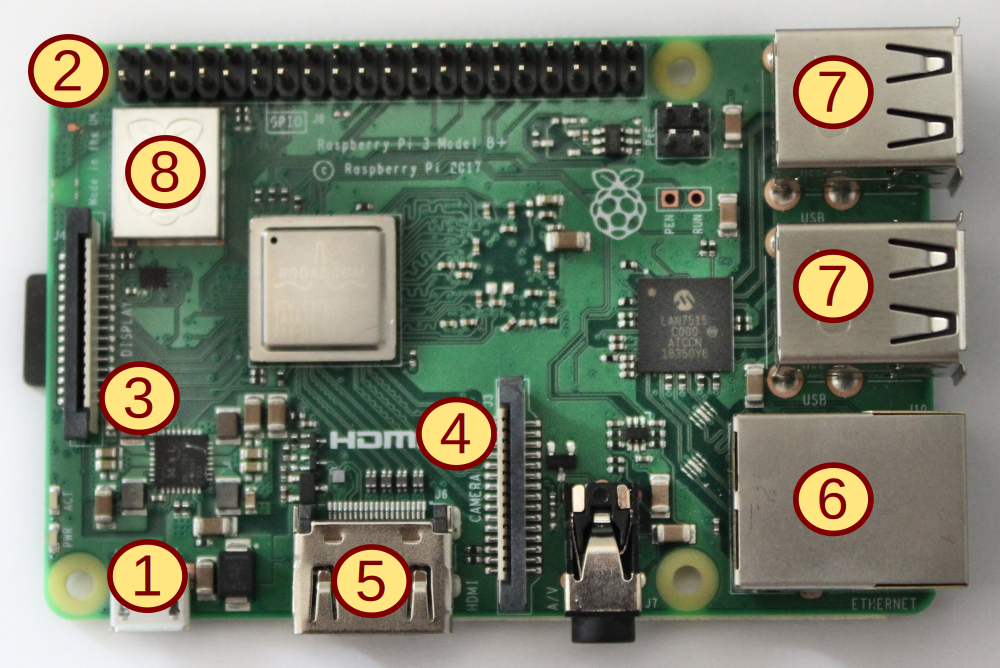
\includegraphics[width=.5\textwidth]{img/raspberry_anschluesse}
\end{center}

\begin{tabularx}{\textwidth}{XX}
        1. Mini-USB-Stromversorgung     &   5. HDMI-Bildschirmanschluss     \\
        2. J8 GPIO-Header               &   6. LAN-Netzwerkanschluss        \\
        3. Display Serial Interface     &   7. USB-Anschlüsse               \\
        4. Camera Serial Interface      &   8. WiFi, Bluetooth              \\
\end{tabularx}

\bigskip
\teilaufgabe
Pins am J8-Header des Raspberry Pi:

\medskip

\begin{tabularx}{\textwidth}{XX}
    \textbf{Stromversorgung:}   &   \textbf{Digital Ein-/Ausgänge:}     \\
    5\,V Power                  &   GPIO                                \\
    3.3\,V Power                &   Pulsweitenmodulation                \\
    Ground (Masse)              &   Asynchron serielle Schnittstellen   \\
                                &   Synchron serielle Schnittstellen    \\
\end{tabularx}

%-------------------------------------------------------------------------------
\loesung{Digitale Komponenten verbinden}
%-------------------------------------------------------------------------------
\teilaufgabe
Untersuchen einer einfachen Schaltung im CircuitJS-Onlinesimulator.

\begin{enumerate}
    \item Am ersten Pin wird mit 22\,mA zu viel Strom gezogen. Es sind maximal
    16\,mA erlaubt,

    \item Aufgrund der unterschiedlichen Stromstärken leuchten die LEDs
    unterschiedlich hell.

    \item Die Stromentnahme an diesem Pin geht auf ca. 5,9\,mA runter.

    \item Die Schaltung zieht ca. 18\,mA vom Raspberry Pi. Da bis zu 50\,mA
    genutzt werden können (wenn die einzelnen Pins 16\,mA nicht überschreiten),
    könnten noch ca. drei weitere LEDs zu je 10\,mA verbunden werden.
\end{enumerate}


\teilaufgabe
Pull-Down-Widerstände dienen dazu, zufällig auftretende Schwankungen des Eingangssignals
durch eingestreute Störungen (sog. parasitäre Induktionen) zu verhindern. Hierzu wird
der zu schützende Eingang über einen Widerstand entweder gegen Masse (Pull-Up) gezogen,
um die Störströme dorthin abzuleiten. Zwar fließt dadurch ein Teil des gewünschten
Eingangssignals ebenfalls Richtung Masse ab. Der Raspberry Pi kann das Signal aber
immer noch zuverlässig erkennen.

Pull-Up-Widerstände dienen hingegen dazu, das Signal eines Sensors mit Active-Low-Logik
zu invertieren. Hierzu wird der Pin mit einem Widerstand auf 3,3\,V und damit auf eine
logische Eins hochgezogen. Solange der Sensor seine Eingangspins kurzschließt, fließt
der Strom über den Sensor ab und der Pi sieht eine logische Null. Sobald der Sensor den
Kontakt unterbricht, fließt der Strom in den Eingangspin, so dass der Pi eine logische
Eins sieht. Würde der Sensor mit Active-High-Logik angeschlossen, wie dies für Sensoren,
die einen Kontakt herstellen statt in zu unterbrechen, würde der Pi genau die gegenteiligen
Werte sehen.

\bigskip
\teilaufgabe
Tastgrad (Duty Cycle) und Frequenz einer mit PWM zum Blinken gebrachten LED:

\begin{itemize}
    \item \textbf{1\,Sek an, 0,5\,Sek aus:}
    Frequenz: 2/3 Hz, Tastgrad: 66\%

    \item \textbf{0,5\,Sek an, 0,5\,Sek aus:}
    Frequenz: 1 Hz, Tastgrad: 50\%
\end{itemize}

\bigskip
\teilaufgabe
Das Signal muss mit einem externen A/D-Wandler abgetastet und als serieller
Datenstrom an den Raspberry Pi übertragen werden.

\bigskip
\teilaufgabe
Eine R2R-Widerstandsleiter realisiert einen einfachen D/A-Wandler mit einer
Handvoll Widerstände. Benannt ist sie nach der Anordnung der Widerstände, wobei
nur die Werte R (ein im Grunde genommen beliebiger Widerstandswert) und 2R (der
doppelte Wert) vorkommen. Indem mehrere GPIO-Ausgänge als die einzelnen Bits
des auszugebenden Werts interpretiert werden, kann durch die R2R-Widerstandsleiter
ein korrespondierendes Analogsignal erzeugt werden.

\bigskip
\teilaufgabe
Sowohl ein npn-Transistor (es gibt nicht viele weitere Arten, die anders funktionieren)
als auch ein Relais funktionieren im Grunde genommen als ferngesteuerte Schalter, die
mit einem Steuersignal vom Raspberry Pi geöffnet oder geschlossen werden können. Der
Unterschied ist, dass ein Transistor dies als Halbleiterelement realisiert, während bei
einem Relais tatsächlich ein mechanischer Schalter bewegt wird. Ein Relais entkoppelt
daher den Steuerstromkreis vollständig vom Arbeitsstromkreis, so dass (das richtige
Bauteil vorausgesetzt), auch sehr hohe Ströme wie z.B. die Netzspannung aus der
Steckdose damit geschaltet werden können. Transistoren eignen sich hingegen nur für
relativ kleine Ströme, da der Arbeitsstromkreis mit dem Steuerstromkreis zusammenfällt.

\begin{center}
    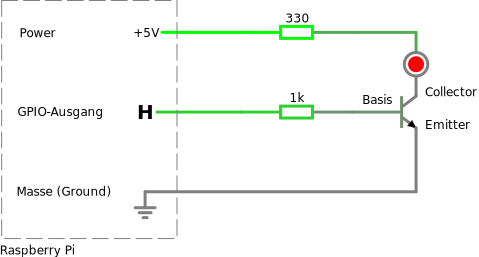
\includegraphics[width=.8\linewidth]{img/led_transistor_circuitjs}
    \bigskip

    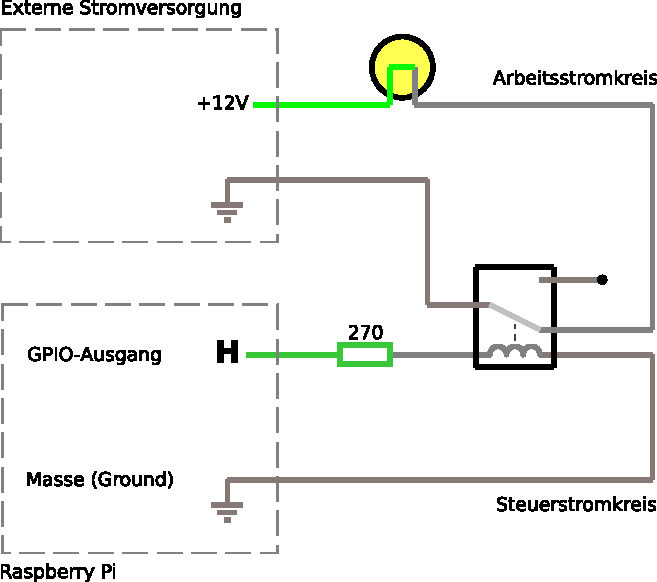
\includegraphics[width=.8\linewidth]{img/led_relais_circuitjs}
\end{center}

\bigskip
\teilaufgabe
Entwurf einer einfachen Transistorschaltung zur Schaltung von 3,3\,V in
Abhängigkeit von einem 5\,V Sensorausgang. Durch entsprechende Vorwiderstände
wird der Gesamtstrom am Transistorausgang auf 2\,mA begrenzt. Die zusätzlich
eingezeichneten Pull-Down-Widerstände verhindern ungewollte Schwankungen des
GPIO-Eingangsignals, indem zufällig auftretende Einstreuungen gegen Masse
abgeführt werden.

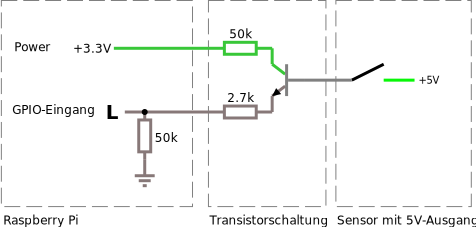
\includegraphics[width=\textwidth]{img/logiklevel_transistor_aufgabe}



%%-------------------------------------------------------------------------------
%\loesung{Serielle Datenübertragung}
%%-------------------------------------------------------------------------------
%\teilaufgabe
%Vergleich der wichtigsten seriellen Übertragungsformate:

%\SerialVergleich{X}

%\bigskip
%\teilaufgabe
%Timingdiagramm zum Übertrag der Zahlen 28 und 3 via SPI:

%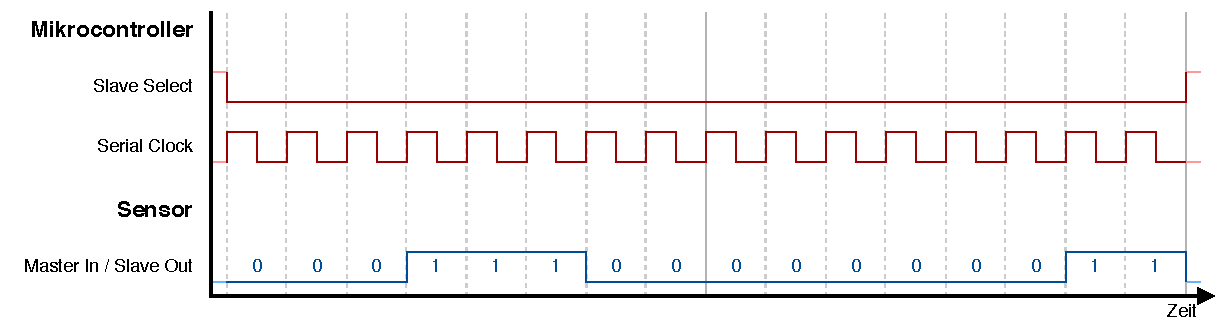
\includegraphics[width=\textwidth]{img/spi_timingdiagramm}

%{
    %\small
    %Der Microkontroller zieht die Slave-Select-Leitung auf Masse runter, um sie
    %zu aktivieren (active-low). Gleichzeitig sendet er auf der Clock-Leitung eine
    %stetige, sich abwechselnde Folge von High- und Low-Signalen zur Synchronisation.
    %Je ein High gefolgt von einem Low bildet dabei einen Takt, während dem der
    %Sensor ein Bit überträgt. Die erste Takthälfte dient dem Sensor dazu, die
    %Datenleitung entsprechend zu setzen, damit der Mikrocontroller den Wert in
    %der zweiten Takthälfte auslesen kann.
%}

%-------------------------------------------------------------------------------
\loesung{Praktische Übung}
%-------------------------------------------------------------------------------
Hierfür gibt es keine Musterlösung. Passen Sie nur auf, dass nichts in die
Luft fliegt. \smiley
